\chapter{Setup Iniziale}


    % INSTALLAZIONE EPIC GAMES LAUNCHER
    \section{Installazione Epic Games Launcher}

        Per installare Unreal Engine e' prima necessario scaricare e installare l'epic games launcher.

        Una volta installato e' necessario aprirlo ed effettuare il login.


    % INSTALLAZIONE UNREAL ENGINE
    \section{Installazione Unreal Engine}

        Dall'Epic Games launcher e' possibile installare Unreal Engine dalla sezione relativa (figura \ref{fig:egl_biblioteca}, cliccare su "Unreal Engine" nell'elenco a sinistra).

        Nella sezione Unreal Engine sono presenti diverse tab tra cui:
        \begin{enumerate}
            \item Tab "Novita'"; contiene le novita' relative alle nuove versioni di Unreal Engine
            \item Tab "Marketplace": contiene contenuti gratuiti e a pagamento gia' pronti da poter inserire all'interno dei propri progetti
            \item Tab "Biblioteca" (figura \ref{fig:egl_biblioteca}): permette di aprire progetti gia' creati, aprire Unreal Engine per creare un nuovo progetto ed installare piu' versioni del motore grafico.

                Il tasto "+" di fianco a "VERSIONI MOTORE" permette di installare una nuova versione di Unreal Engine.

                Durante l'installazione e' possibile specificare nelle opzioni cosa installare per ridurre le dimensioni dell'installazione.

                \begin{suggestionbox}
                    Tra le opzioni e' possibile specificare anche di scaricare l'"Engine Source" e i "simboli dell'editor per il debug" per fare il debugging del codice C++:
                    quest'ultima opzione e' molto pesante (50 GB) ma permette di eseguire il debugging senza andare incontro ad ostacoli
                    (messaggi del tipo "impossibile visualizzare la risorsa, simboli non trovati").
                \end{suggestionbox}

                A fine installazione e' possibile cliccare la freccia a destra del pulsante "Avvia" per modificare le impostazioni di Unreal Engine o disinstallarlo.

                Sotto alla sezione "VERSIONI MOTORE" e' presente un elenco con tutti i progetti creati.

                Piu' in basso e' possibile vedere gli oggetti acquistati o riscattati gratuitamente dal marketplace.

        \end{enumerate}


    % IDE PER C++
    \section{IDE per C++}

        Per programmare in C++ e' necessario installare un IDE.

        Alcune valide opzioni sono:
        \begin{itemize}
            \item \href{https://visualstudio.microsoft.com/}{Visual Studio} della Microsoft
            \item \href{https://www.jetbrains.com/lp/rider-unreal/}{Rider for Unreal} della JetBrains
        \end{itemize}

        Per maggiori informazioni guardare il capitolo \nameref{chapter:cpp} a pagina \pageref{chapter:cpp}.


    % CREARE UN PROGETTO
    \section{Creare un progetto}
        Quando si lancia il motore grafico, dopo aver cliccato sul pulsante "Avvia", apparira' il project browser.

        Dal project browser (figura \ref{fig:ue_project_browser}) e' possibile:
        \begin{itemize}
            \item Aprire o creare nuovi progetti
            \item Dalle categorie e' possibile selezionare un template del progetto che si vuole creare
            \item Dopo aver selezionato un template, si puo' selezionare se il progetto usera' Blueprint o C++, la qualita' dei preset, se inserire i contenuti iniziali e se attivare il raytracing

                \begin{notebox}
                    I Blueprint permettono di programmare in modo visuale (collegando assieme blocchi mediante l'interfaccia grafica) azioni
                    da eseguire in base agli eventi lanciati ed esposti dal codice C++ di Unreal Engine oppure in base ad altri eventi personalizzati.

                    E' possibile mescolare Blueprint e codice C++ all'interno di un progetto.
                \end{notebox}

            \item Impostare il nome del nuovo progetto e crearlo.
        \end{itemize}

        \begin{suggestionbox}
            Personalmente preferisco prima creare i progetti da Unreal Engine e successivamente aprire i progetti
            gia' creati facendo doppio click sul file .uproject contenuto nella cartella del progetto:
            in questo modo non e' necessario ogni volta aprire l'Epic Games Launcher, avviare il project browser e selezionare il progetto da aprire.
        \end{suggestionbox}


    % FIGURE

    \begin{figure}[h]
        \caption{Epic Games Launcher: Biblioteca}
        \centering
        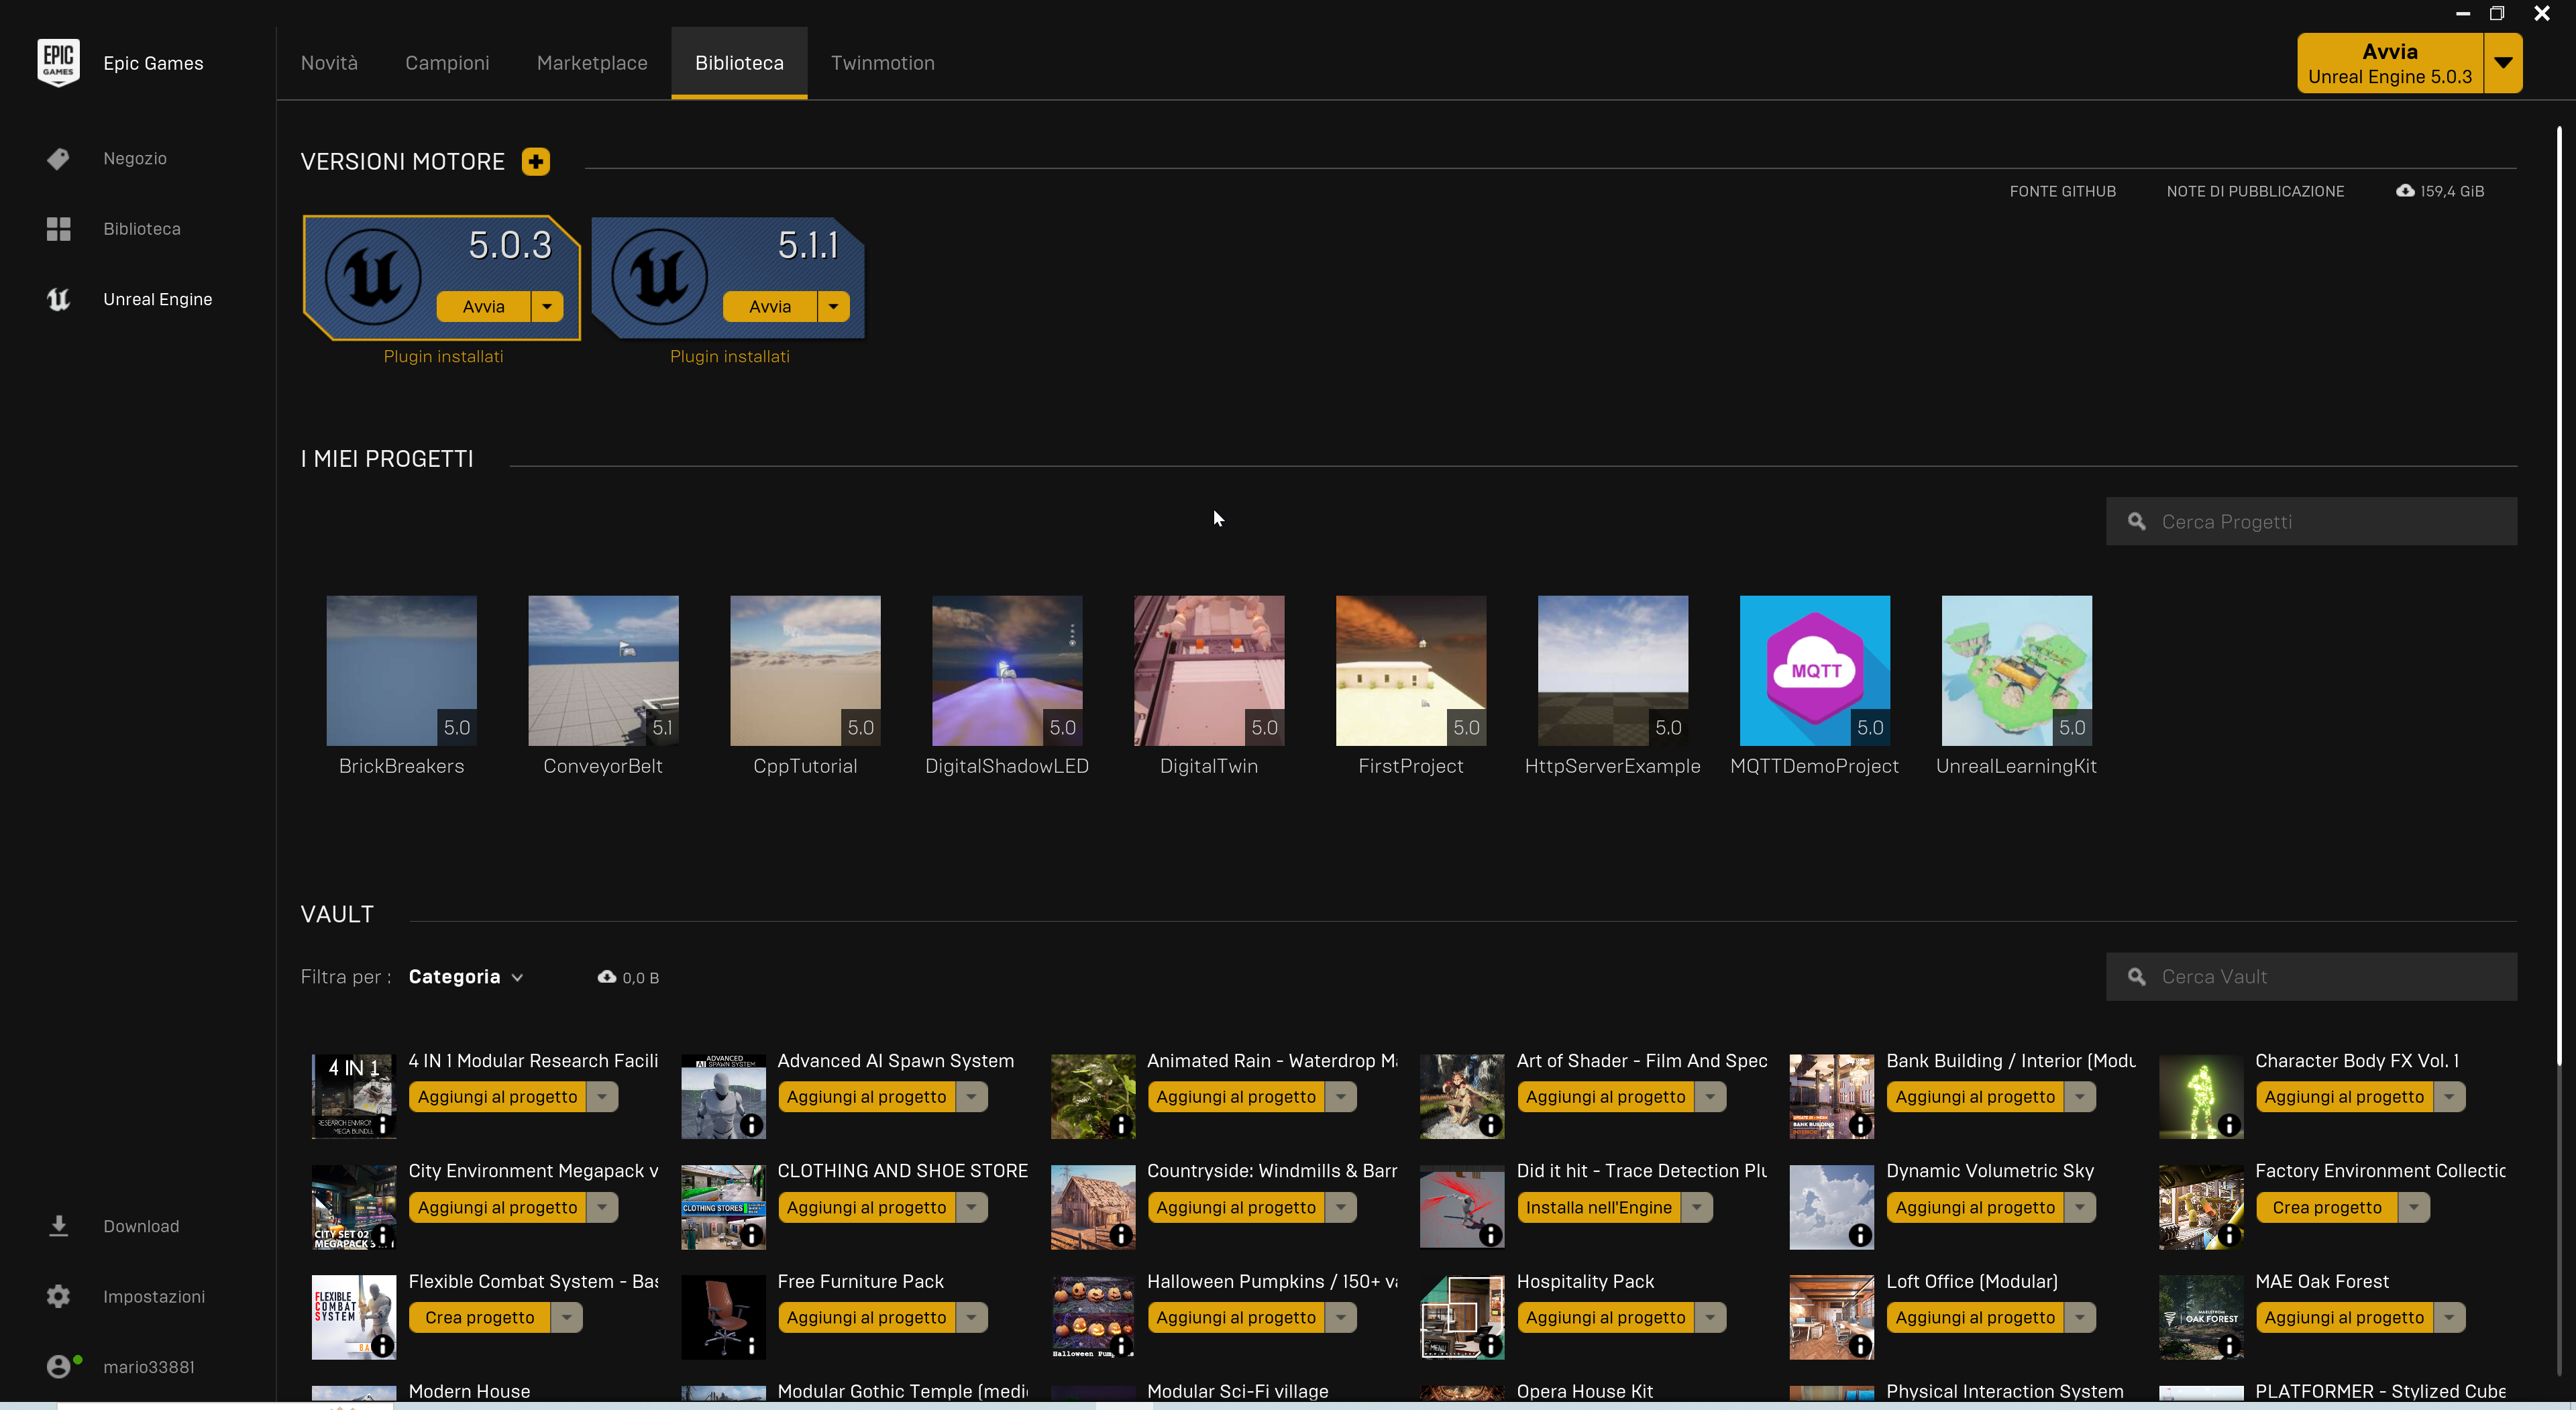
\includegraphics[width=\textwidth]{epicgameslauncher_biblioteca}
        \label{fig:egl_biblioteca}
    \end{figure}

    \begin{figure}[h]
        \caption{Unreal Engine: Project Browser}
        \centering
        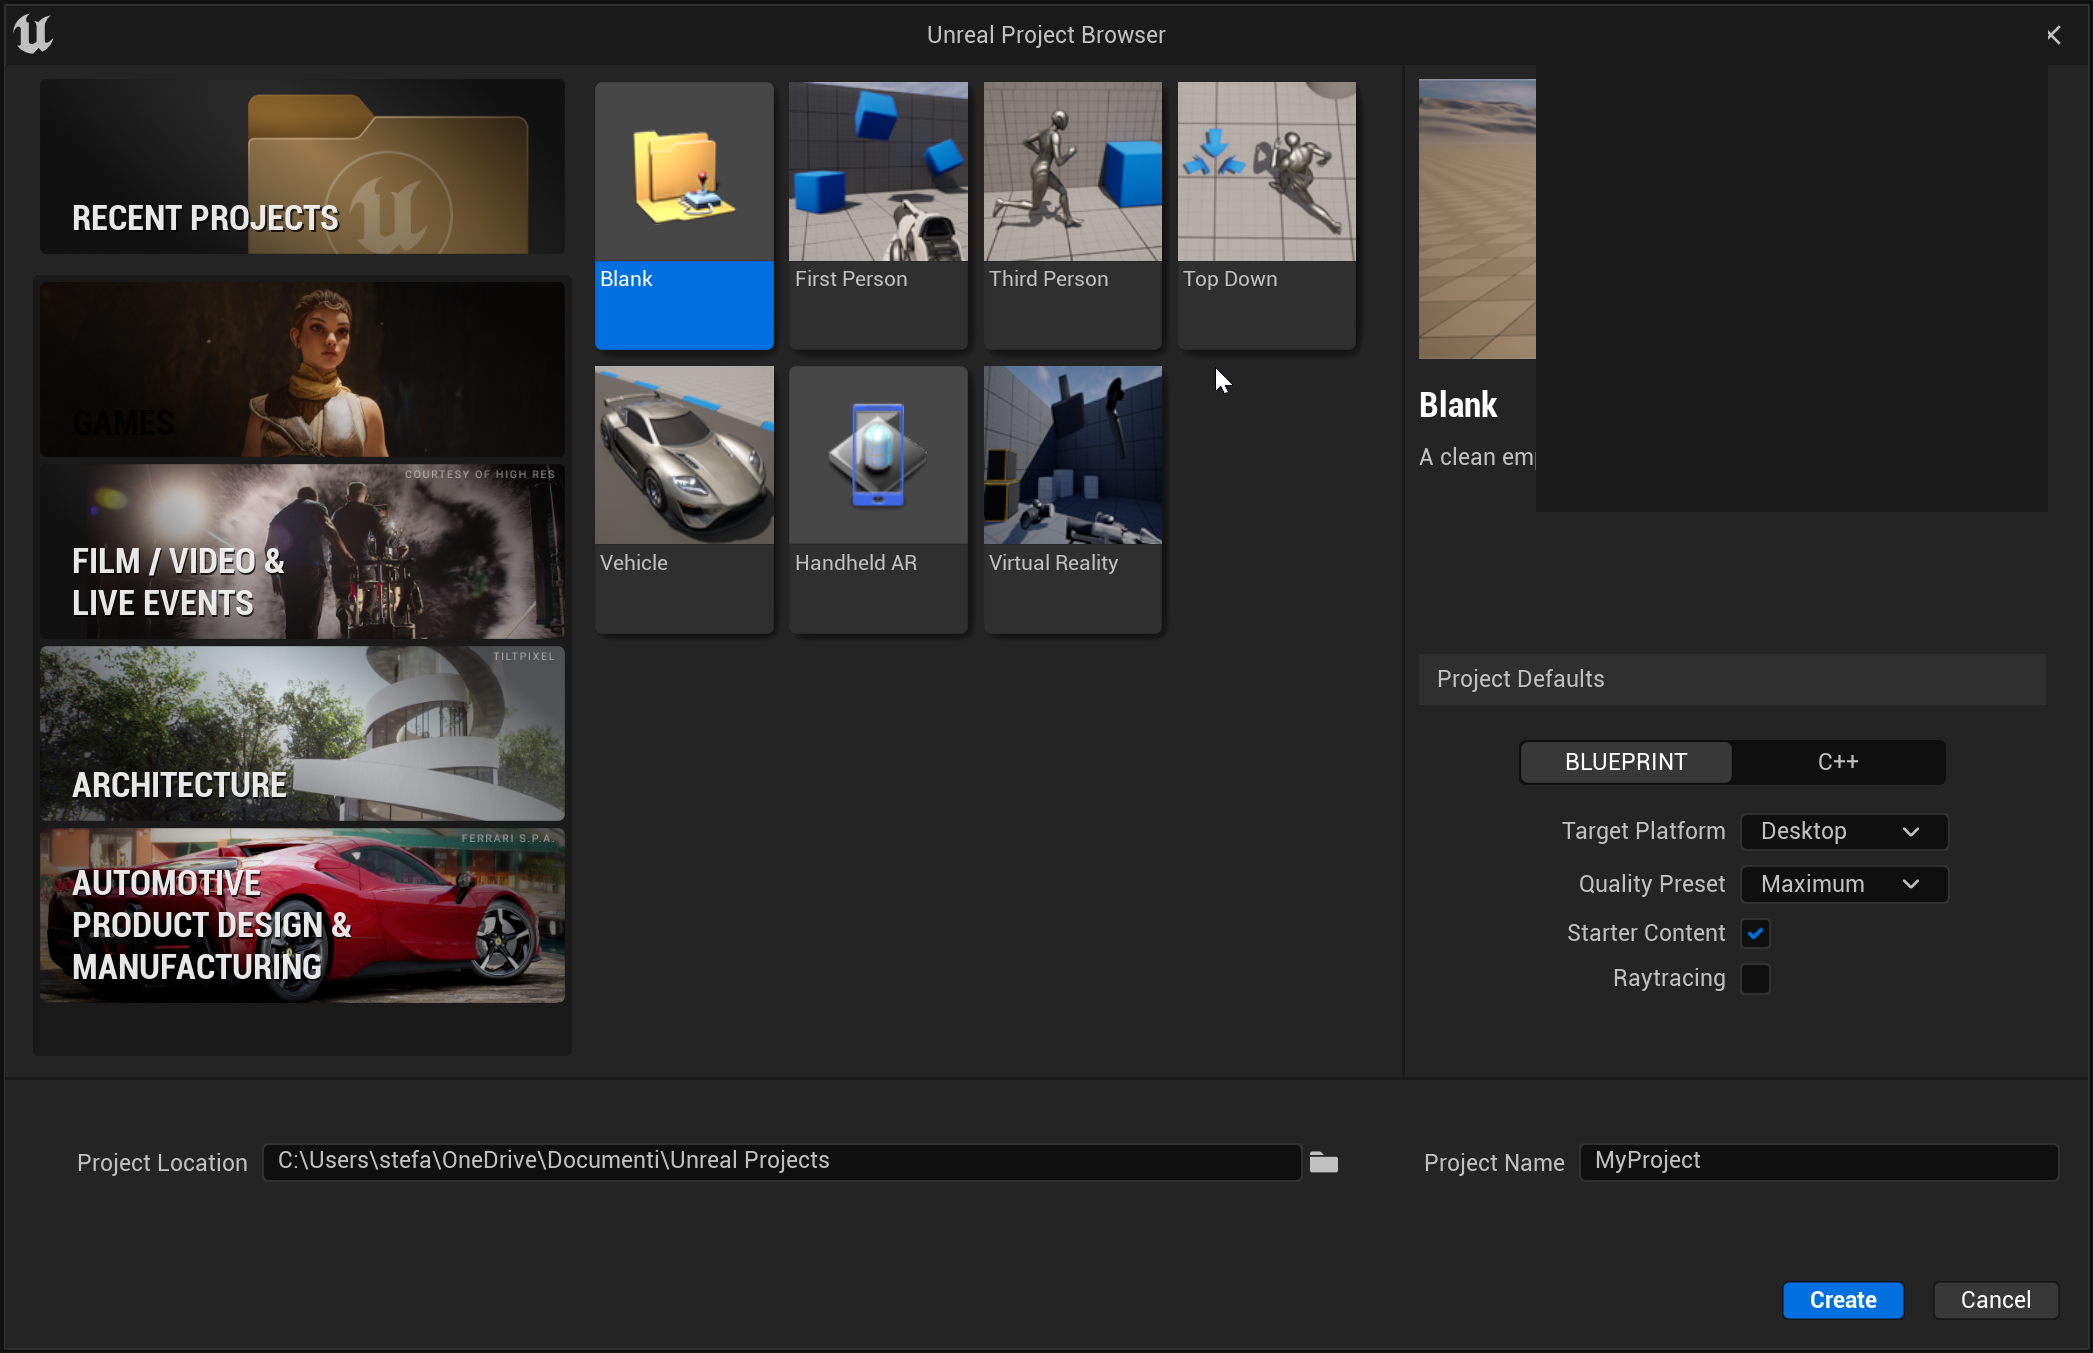
\includegraphics[width=\textwidth]{unreal_engine-project_browser}
        \label{fig:ue_project_browser}
    \end{figure}
